\forceindent The observation of the first multiply-imaged, gravitationally lensed supernova (SN) in 2014, SN ``Refsdal", 
was a critical step forward for the SN cosmology community (Figure 1; \citet{Kelly:2015a}). As light from a distant
source passes through a gravitational lens, each subsequent image will appear to the observer delayed relative to the 
unlensed travel time. If the lensing potential is well known, then the {\bf time delay measurement  provides a direct constraint on
the Hubble constant that is completely independent of the local distance ladder.} There are certain degeneracies associated with
obtaining these constraints directly from time delays, which are broken in the case of a Type 1a "standard candle" SN. The very 
first multiply-imaged Type 1a SN, was discovered by \citet{Goobar:2016} (SN iPTF16geu), but attempts to constrain the time delays have been 
only moderately successful citing the need for a comprehensive mechanism that includes microlensing effects as a primary source of uncertainty 
\citep{More:2016}. We propose to perform a complete reanalysis of SN Refsdal in order to refine our constraints on the lensing parameters 
and define a rigorous methodology for use in a parallel analysis of . We will improve upon previous work by making substantial improvements 
to the photometry, and including the significant yet previously ignored effects of microlensing. Additionally, we will produce an open-source software 
package in the course of this work, optimized specifically for multiply-imaged SNe. 

\begin{figure}[h]
\centering
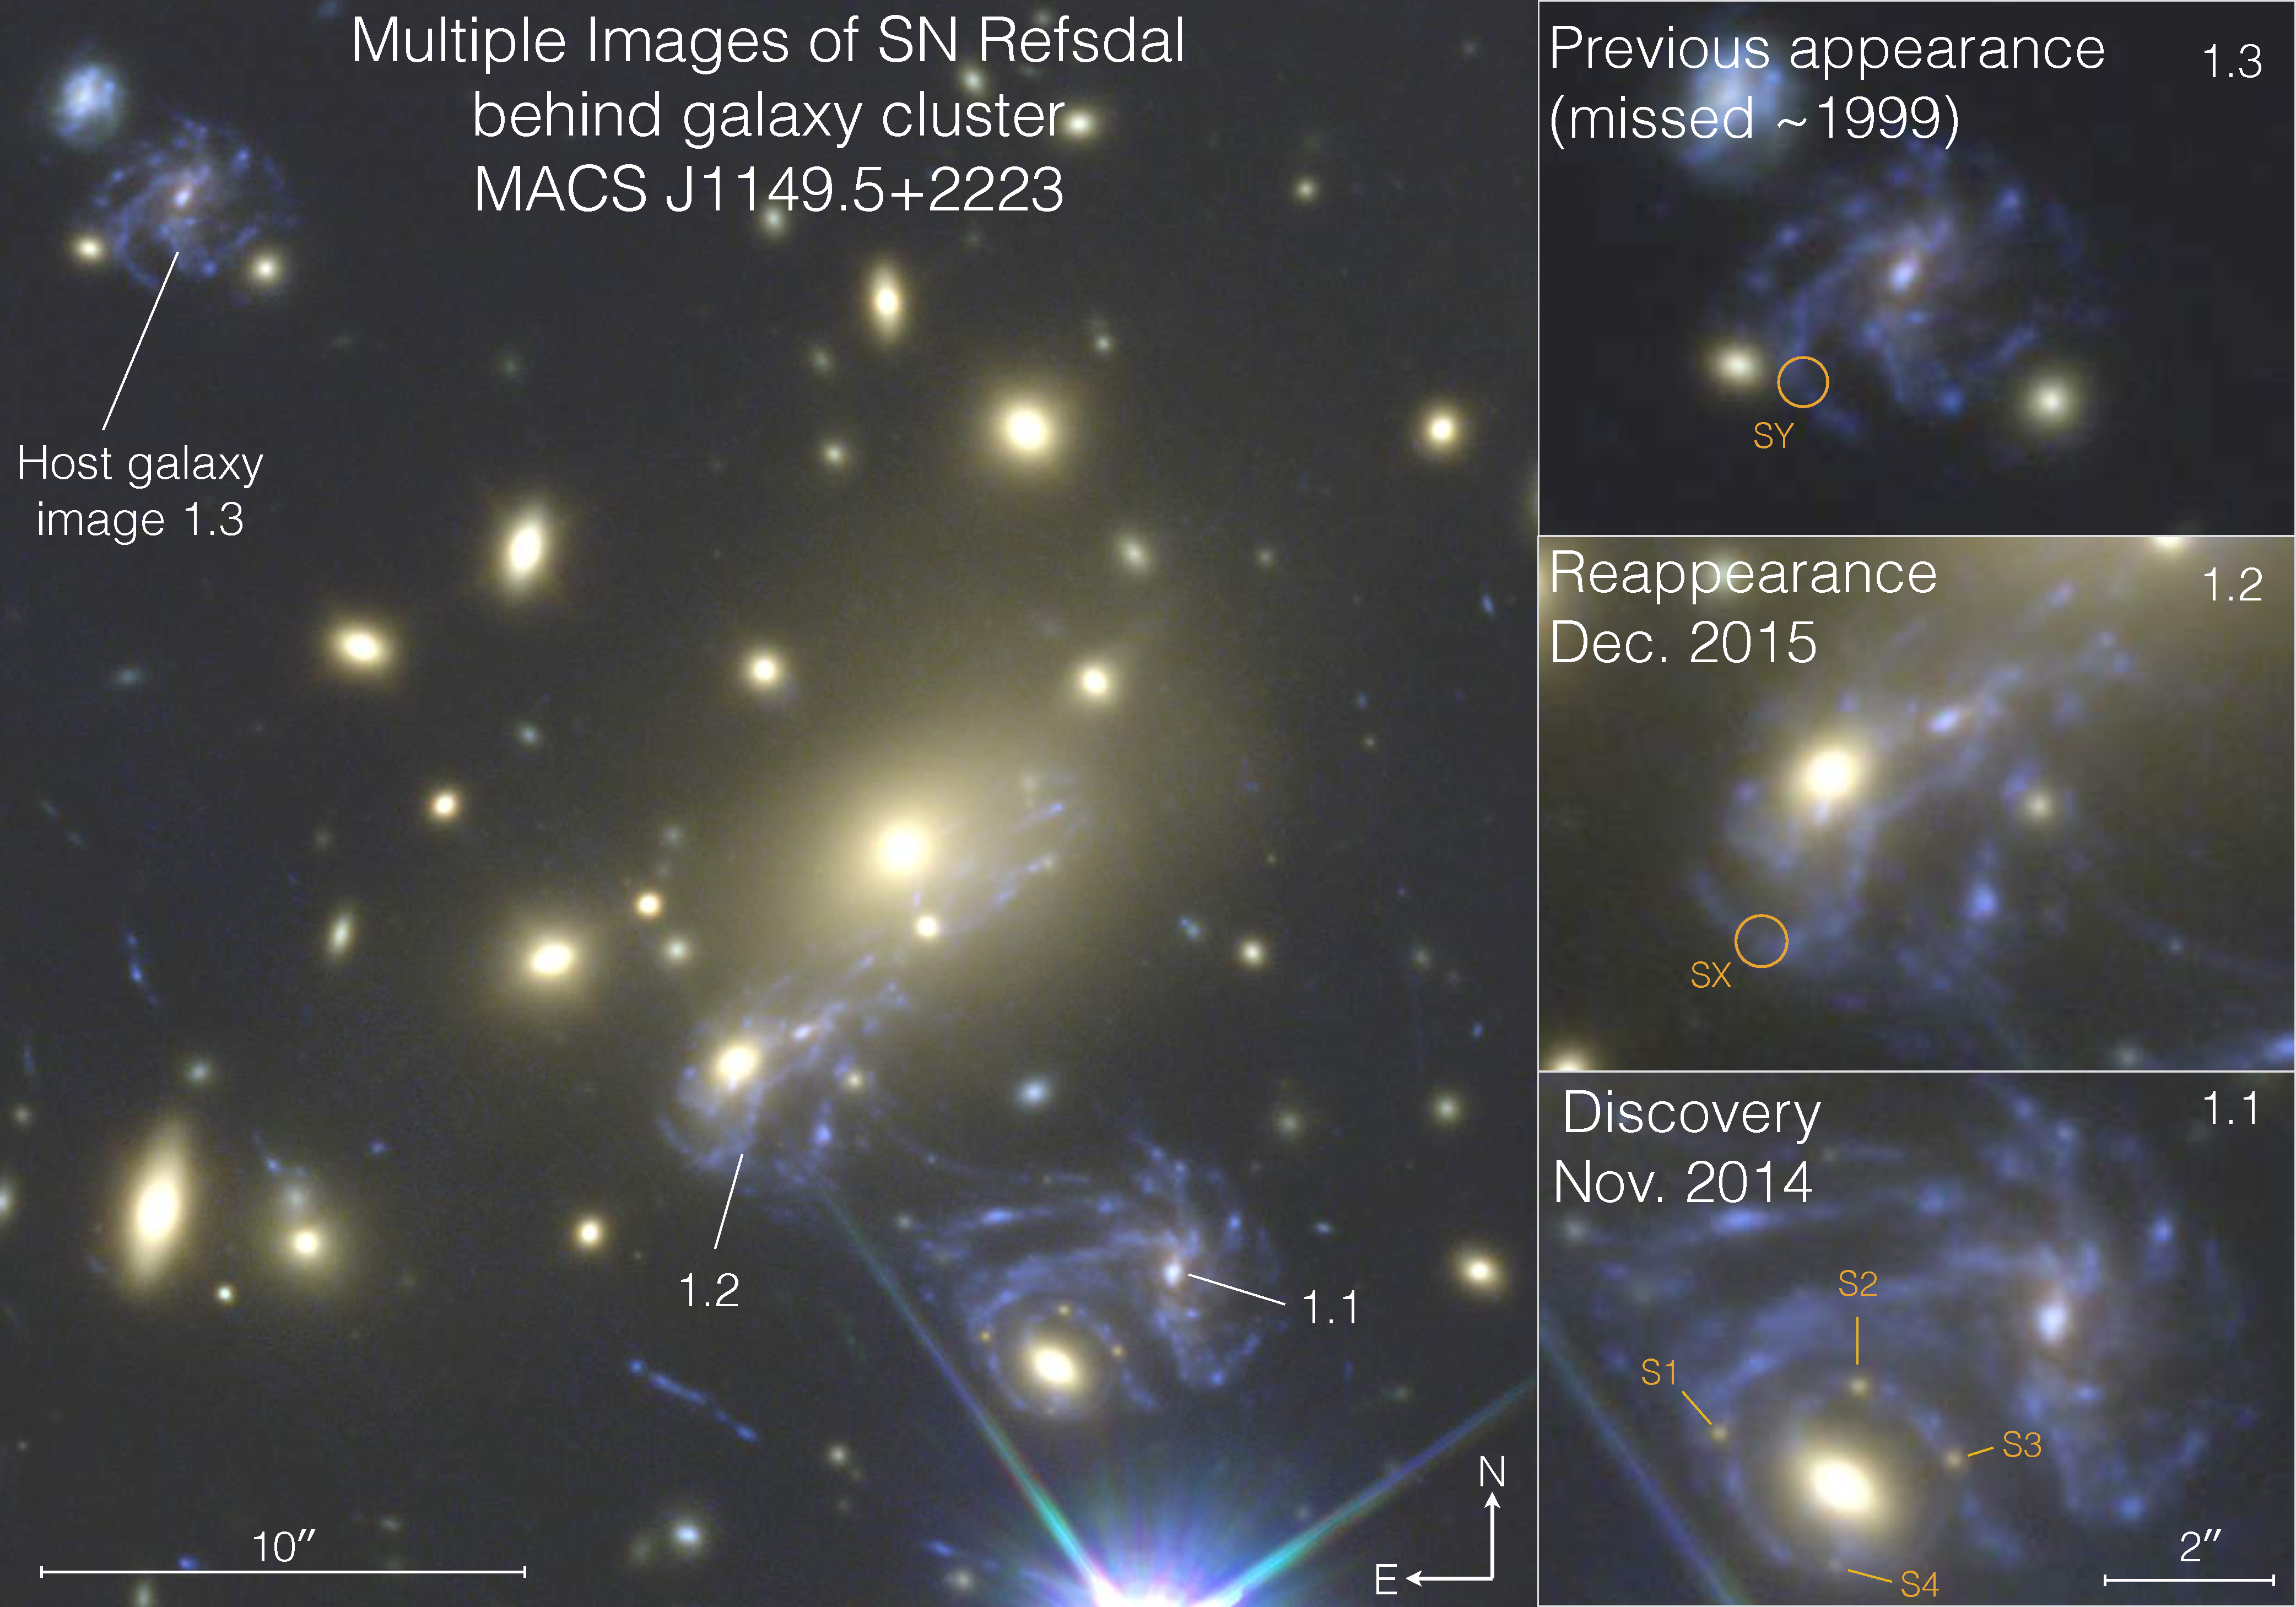
\includegraphics[width=0.65\textwidth]{FIG/refsdal_rodney.pdf}
\caption{
MACS J1149.6+2223 field, showing the positions of the three primary
images of the SN Refsdal host galaxy (labeled 1.1, 1.2, and 1.3). SN
Refsdal appears as four point sources in an Einstein Cross
configuration in the southeast spiral arm of image 1.1 \citep{Rodney:2016}}
\end{figure}

\noindent {\bf A New Software Package:}

\textbf{The next decade is expected to yield observations
of over 100 lensed SNe} that will require analysis \citep{Oguri:2010},
yet \textbf{there is no public software package for analyzing multiply-imaged SNe.}
The lack of a standard resource leaves researchers to write and implement their 
own ad hoc programs, which will become increasingly inefficient as the number of
observed lensed SNe increases. In the course of this work, 
we are producing an open-source software package written in Python for use in this and future SN analysis.

There are currently two software packages that form the basis 
of this product: Supernova Cosmology (SNCosmo), and Python Curve Shifting (PyCS) used for quasars. Unlike quasars, 
SNe of a given class always have consistent and well-known light curve shapes. This will allow for physically motivated, 
less flexible models that will be more likely than PyCS to correctly identify SN 
microlensing effects and produce simpler time delay measurements. By allowing certain constraints to float as free 
parameters, these models will also produce best-fit synthetic light curves from which time delays, magnifications, 
SN class, and redshift can be derived. By simulating large numbers of SNe with these synthetic light curves, we will 
be able to quantify the accuracy and efficiency of the software.

\bigskip

\noindent {\bf Microlensing Effects:}

Microlensing refers to small-scale gravitational lensing
perturbations due to massive objects along the light path of any one image of a
multiply-imaged SN. The effect of microlensing is to cause distortions in the SN light
curves that significantly limit the precision that can be achieved in the measurement of 
their time delays. After the discovery of Refsdal in 2014, subsequent work was done to 
classify the SN \citep{Kelly:2016}, as well as measure time delays and magnification
ratios \citep{Rodney:2016}. These previous analyses completely ignored microlensing; 
therefore we will \textbf{fully analyze the effects of microlensing on a multiply-imaged SN for the first time.}

Lensed SNe are affected by microlensing caused both by transverse motion of stars in the lensing galaxy (type 1), and as the
expanding photosphere of a SN interacts with an increasing volume of the caustic web (type 2). The latter form, which precipitates
microlensing effects described by \cite{Dobler:2006} that can cause fluctuations of $\sim$0.2 to $>$0.5 magnitude, is unique 
to lensed SNe and has never been fully classified or considered in lensed SN analysis. Therefore, an algorithm will be developed 
following the methodology of \cite{Dobler:2006} and released as a component of the open-source software packaged being 
developed in the course of this work. In preparing this proposal, we have already used flexible functions to preliminarily 
measure the effects of the type 1 microlensing (Figure 2), and it's \textbf{clear that microlensing must be taken into account} in order
to ensure accurate time delay and magnification measurements. 


\begin{figure}
\centering
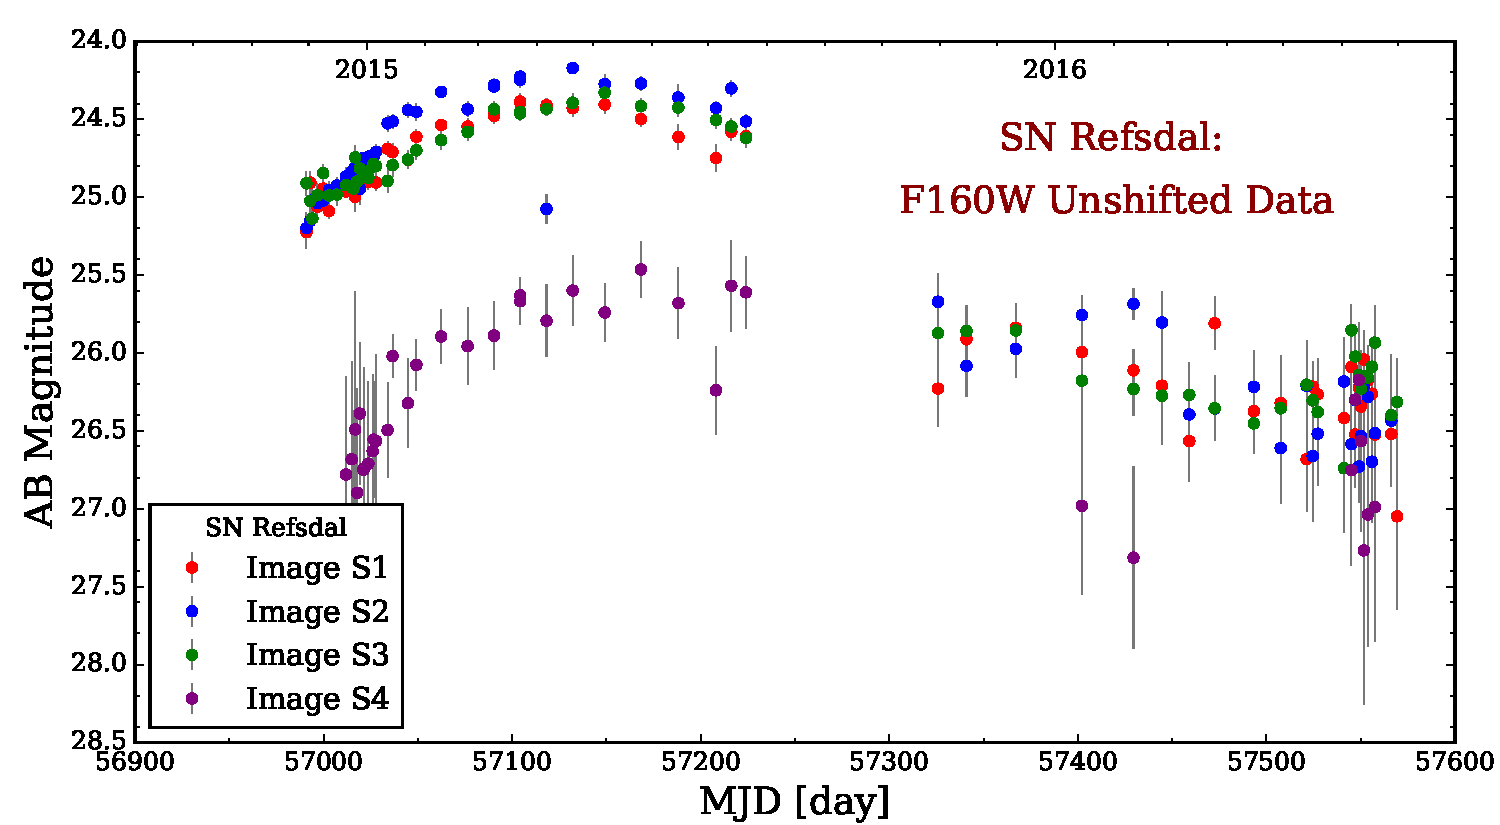
\includegraphics[width=.7\textwidth]{FIG/points_plot_2017.pdf}
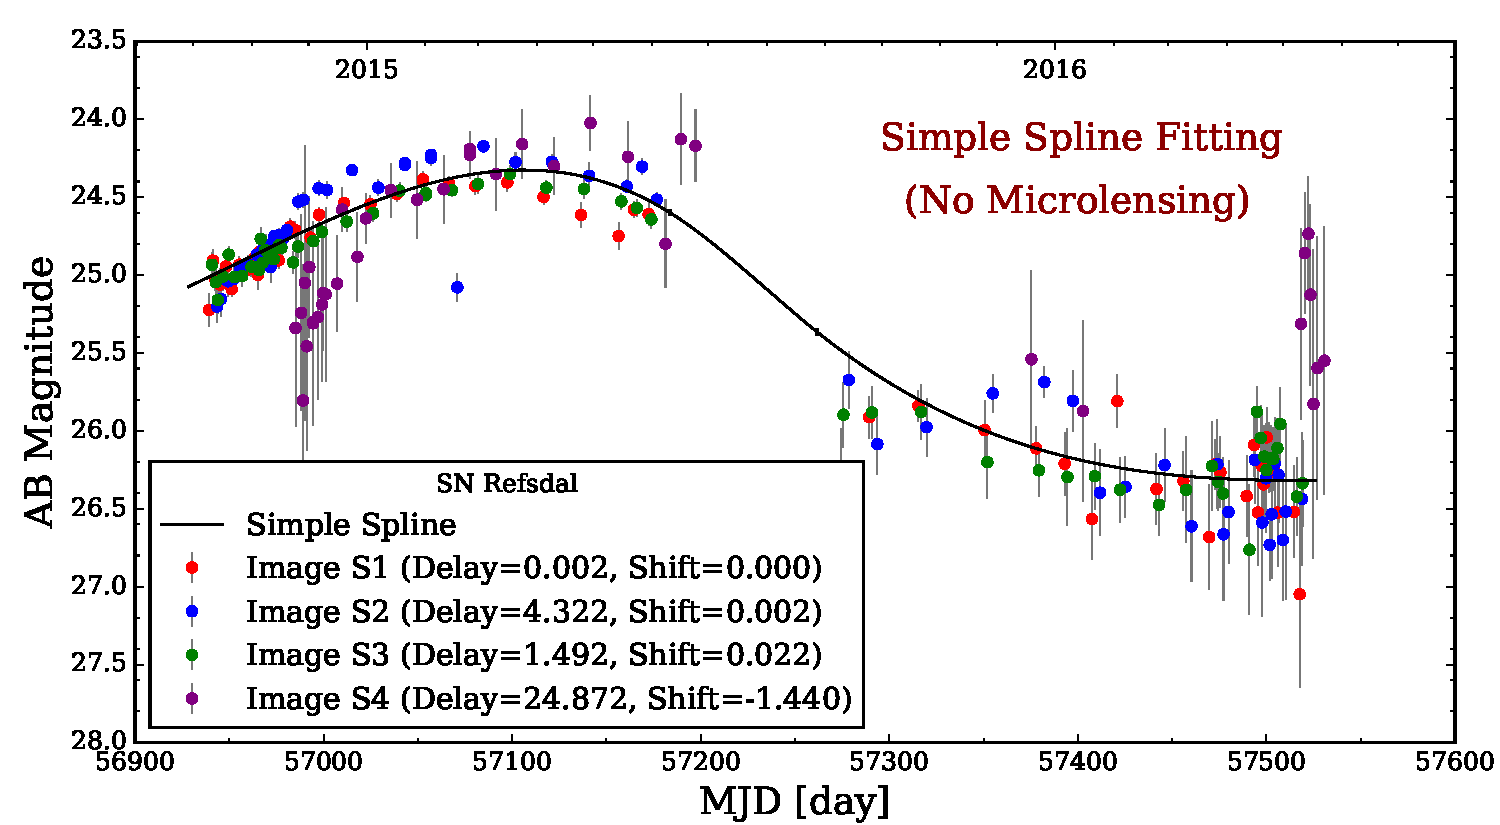
\includegraphics[width=.7\textwidth]{FIG/refs_plot_2017.pdf}
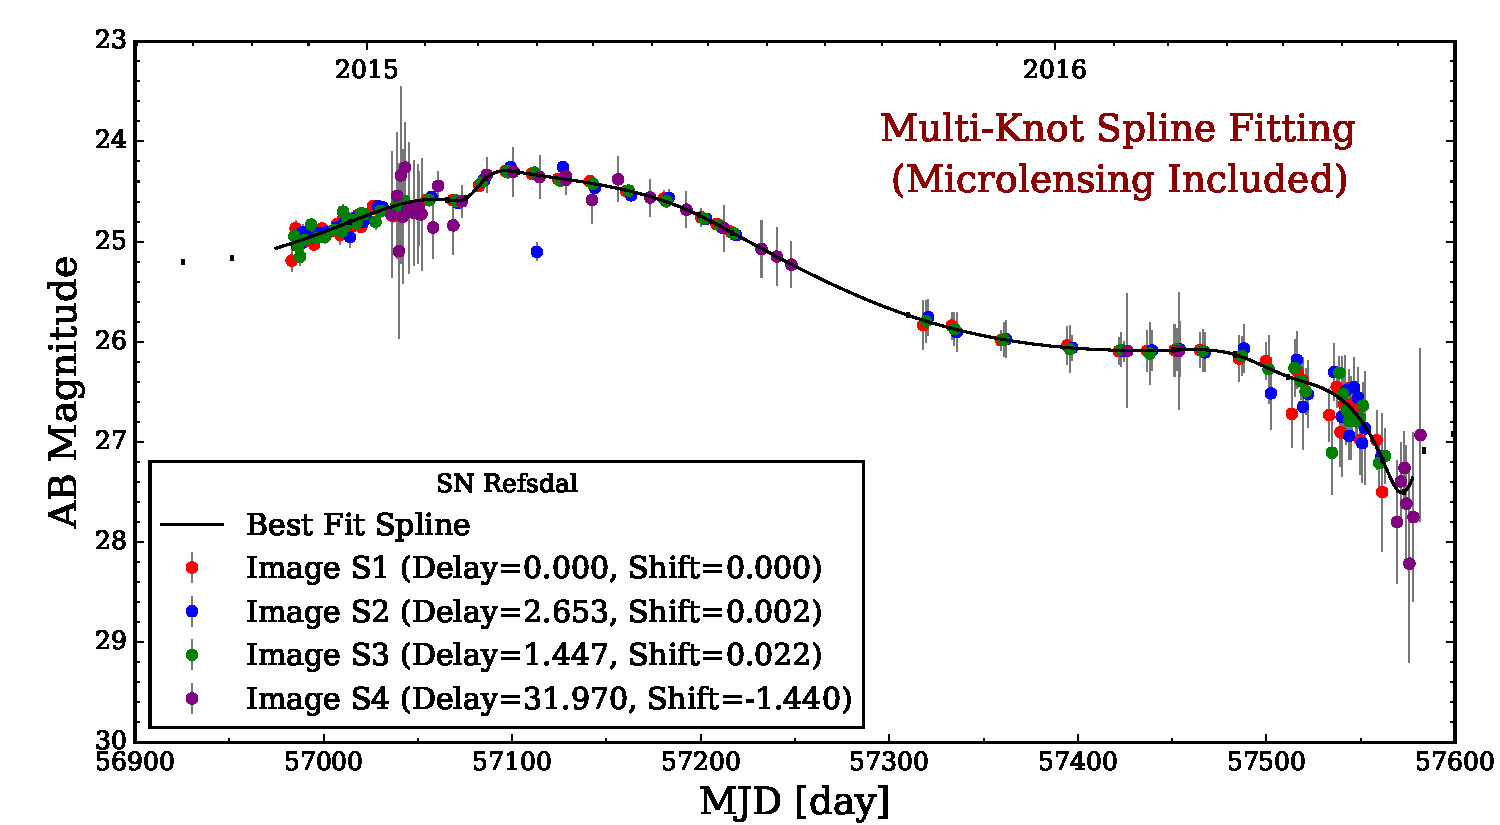
\includegraphics[width=.7\textwidth]{FIG/spline_plot_2017.pdf}
\caption{(Top) HST F160W data representing the four images of SN
Refsdal (Figure 1), with no lensing or time shifts. (Middle) Method of
fitting the SN Refsdal light curves from Rodney et al. 2016, which did
not consider microlensing effects. (Bottom) Preliminary results from 
this work using a multi-knot spline to fit the data. This method 
includes microlensing effects, which leads to a slight adjustment in 
time delay measurements. }
\end{figure}

\bigskip

\noindent {\bf Improving Photometry:}
 
Measuring photometry with a single photometric tool, as was done in \cite{Rodney:2016}, means that potential systematic errors may be disregarded. 
As a check against systematic biases, our reanalysis will use both the \textit{PythonPhot} and the \textit{DOLPHOT} package to 
perform photometric measurements. We will also measure the photometry in single-exposure images, allowing us to check for any deviations 
at very short timescales, indicative of very rapid microlensing events. \cite{Rodney:2016} measured flux using a single empirical 
point-spread function (PSF) fixed in time, derived from standard stars. However, as we know that the HST PSF does undergo 
subtle variations due to telescope ``breathing" (\textbf{CITE}), our re-analysis will use foreground stars within the MACS1149 imaging 
datasets to define a variable PSF model. \textbf{The reduction of systematic biases in the photometry and our improvements to the 
PSF will provide drastically ameliorated flux calculations, which in turn will increase the accuracy and precision of time delay 
measurements in our reanalysis.}




